\documentclass[12pt,a4paper]{article}
\usepackage{Diplo}

\usepackage[left=3cm,right=1.5cm,
top=2cm,bottom=2cm]{geometry}

\usepackage{comment}
\usepackage{hyperref}
\usepackage{caption}
%\captionsetup[figure]{font=normalsize,labelfont=normalsize}
%\graphicspath{{../pics/}}
\renewcommand{\rmdefault}{cmr}
\renewcommand{\sfdefault}{cmr}
\renewcommand{\ttdefault}{cmr}



\begin{document}
\newpage
\begin{abstract}
	{}
	

\end{abstract}

\newpage
\tableofcontents



\newpage
\section{Введение}
В современном мире — мире информационных технологий — многие компании сталкиваются с проблемой утечки конфиденциальной информации.
Причиной такой утечки может стать не только атака извне, но и действия сотрудников компании, нарушающих коммерческую тайну.
Совокупность технологий предотвращения утечек конфиденциальной информации и технических устройств, обеспечивающих это предотвращение, называемая Data Leakage Prevention (далее, DLP), позволяет не только предотвращать, но и расследовать случаи кражи данных.
Так, на рабочем устройстве сотрудника может быть установлено специализированное ПО, осуществляющее логирование действий пользователя или запрещающее выполнять некоторые действия: в частности, может быть заблокирован доступ к сети Интернет, использование съемных USB-накопителей и т.д.
Однако такие системы не могут запретить сотруднику воспользоваться цифровой камерой, чтобы получить снимок конфиденциального документа, содержимое которого отображается на экране монитора.
Сделав снимок экрана, злоумышленник обходит систему логирования, что усложняет расследование факта утечки. 
Цифровые камеры современных смартфонов способны делать снимки высокого качества за короткое время, из-за чего становится сложнее осуществлять контроль за такого рода утечками.
Один из подходов, упрощающих расследование утечек, состоит во встраивании дополнительной информации в изображение, выводимое на экран.
Такая информация может содержать в себе идентификационные данные пользователя устройства.
Если впоследствии «украденное» изображение окажется в публичном доступе, внедренная дополнительная информация поможет выяснить, какой именно пользователь допустил утечку.

Встраивание дополнительных данных в изображение относится к технологии внедрения цифровых водяных знаков (далее, ЦВЗ).
В настоящий момент технология ЦВЗ широко применяется в области защиты авторских прав цифровых данных различных форматов: изображений, фильмов, музыкальных файлов.
Далее будем отождествлять понятия ЦВЗ и \textit{цифровая метка}, а процесс встраивания ЦВЗ в изображение будем называть \textit{маркирование изображения}.

На рисунке~\ref{fig:scheme} представлена общая схема использования ЦВЗ [].
Система маркирования изображений предполагает наличие двух алгоритмов: алгоритма встраивания ЦВЗ и алгоритма извлечения ЦВЗ. Алгоритму встраивания ЦВЗ на вход подается изображение и цифровая метка, зависящая от передаваемого сообщения.
В некоторых системах маркирования изображений также используются схемы шифрования для защиты цифровой метки.
В таких системах при встраивании ЦВЗ задействуется также криптографический ключ.
Результатом работы алгоритма встраивания является маркированное изображение.
\begin{figure}[h]
	
	\centering
	
	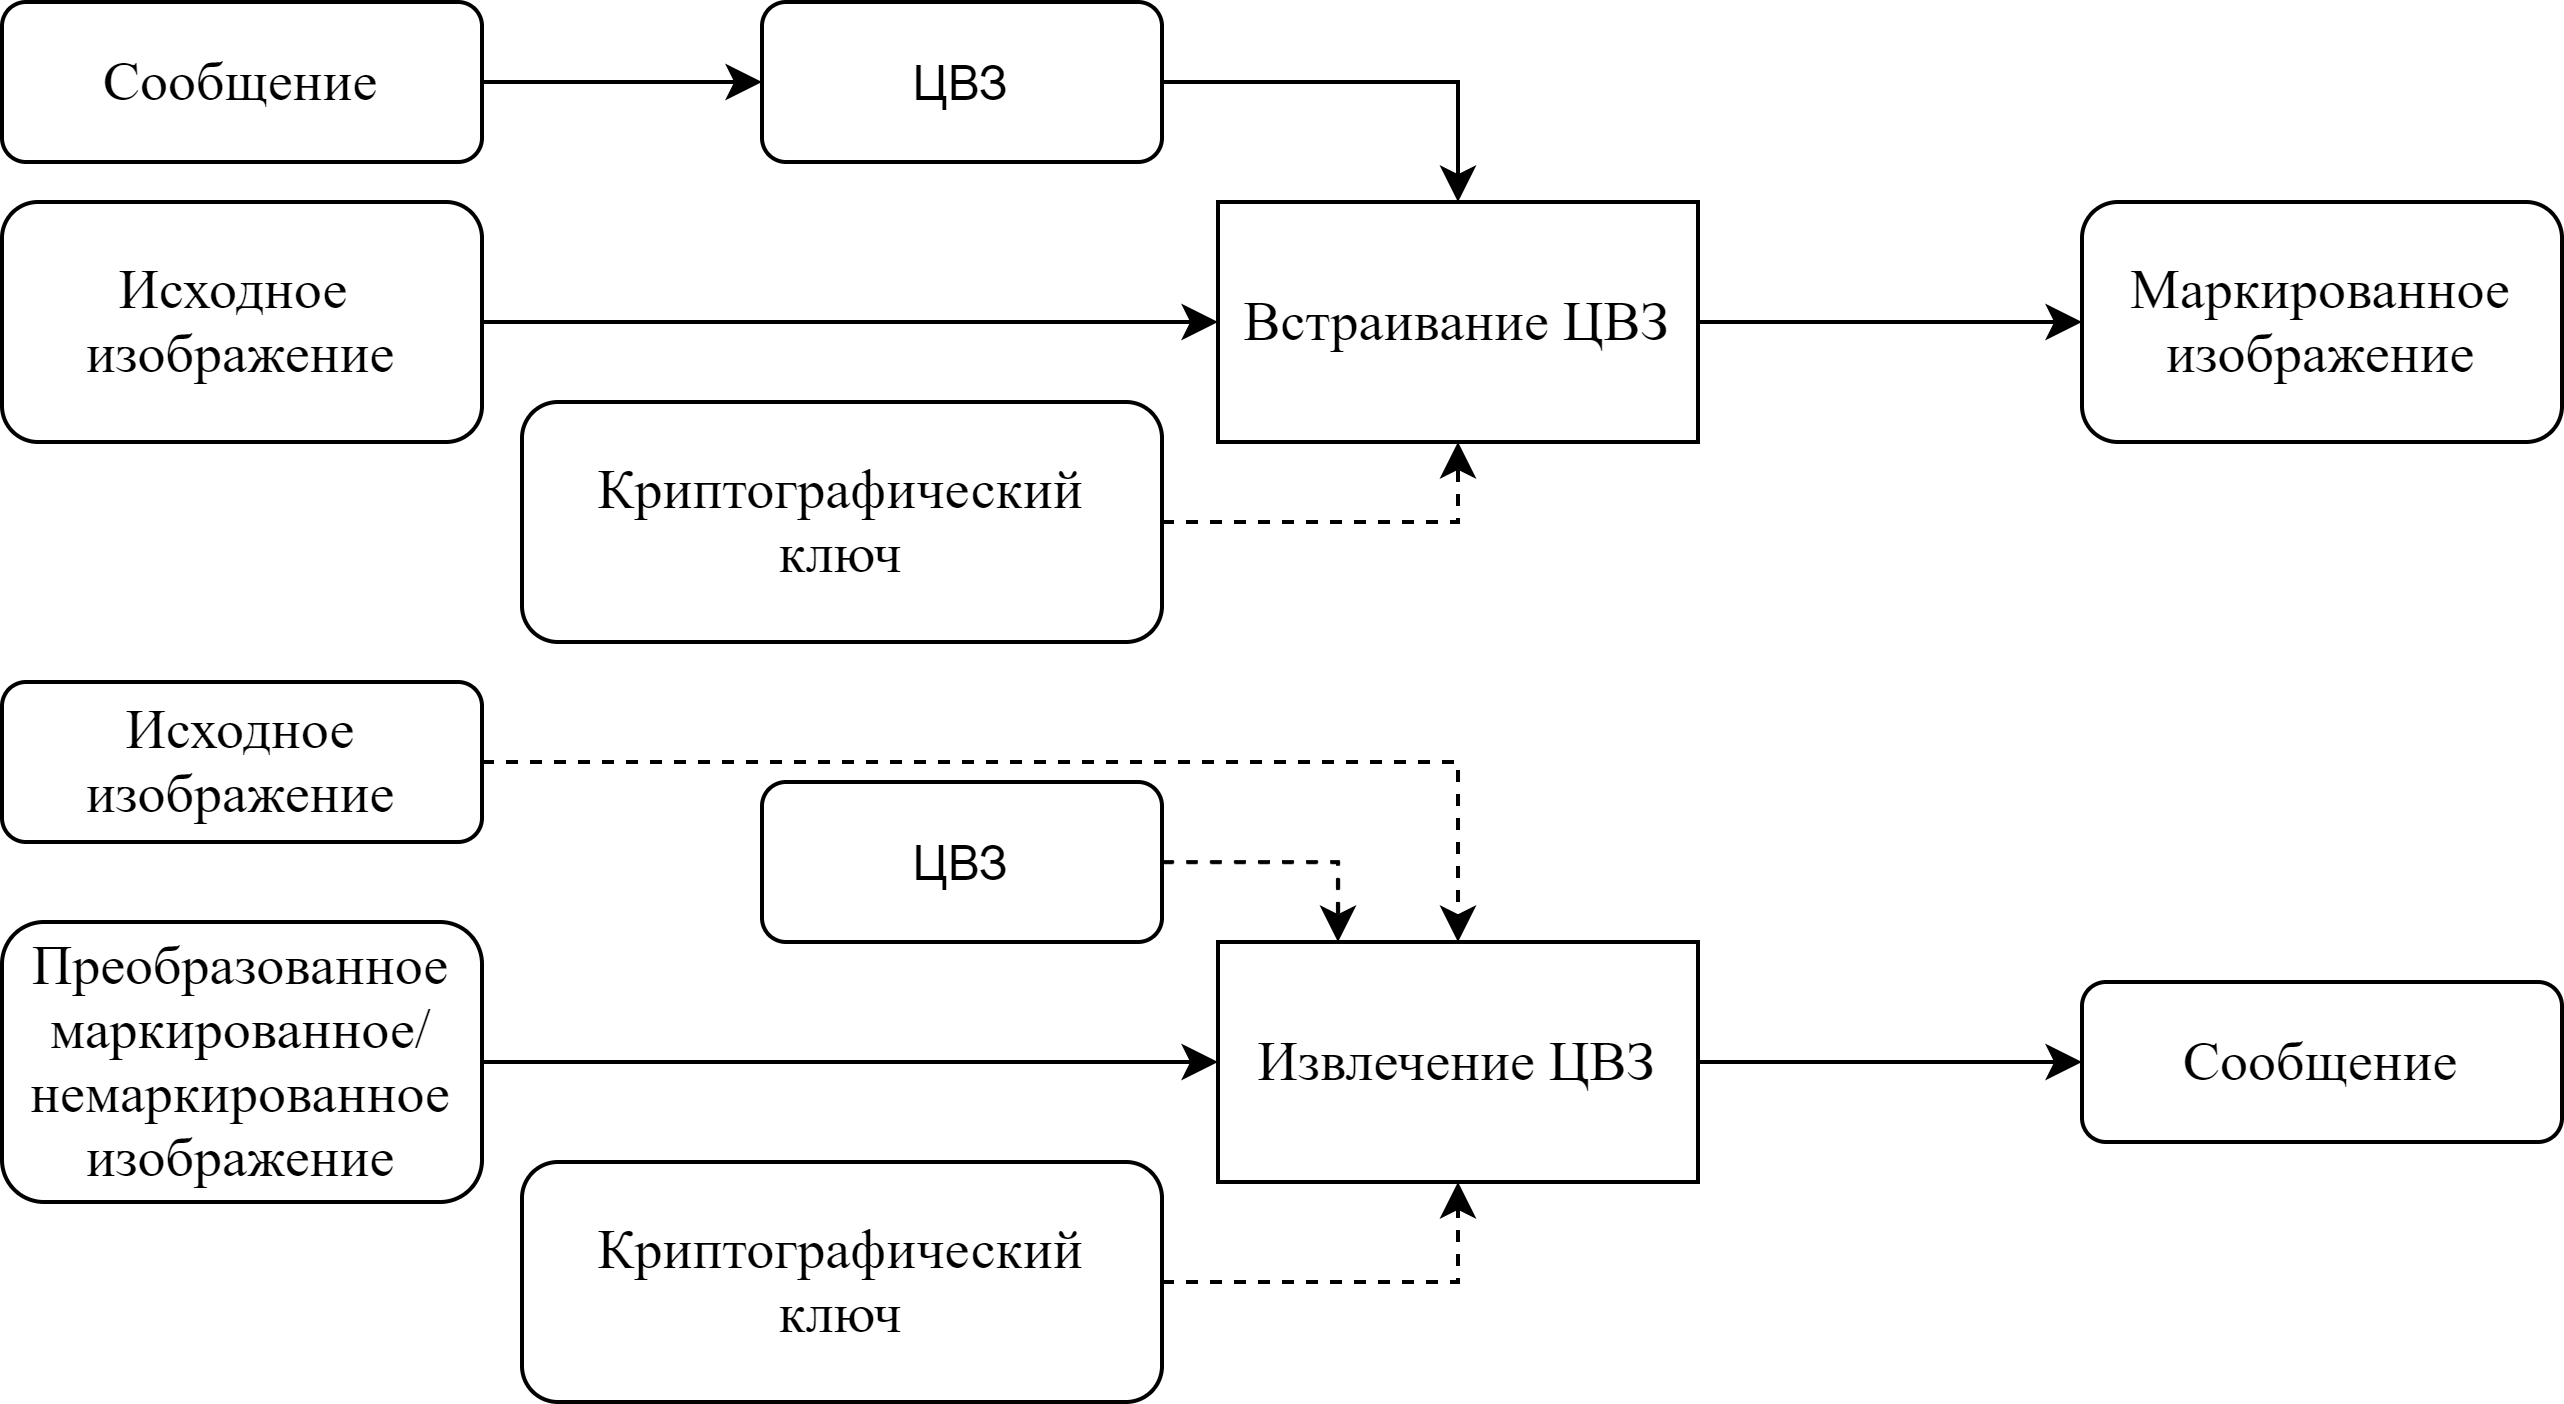
\includegraphics[width=1.0\linewidth]{Scheme.png}
	
	\caption{Общая схема использования ЦВЗ}
	
	\label{fig:scheme}
	
\end{figure}
Процесс извлечения ЦВЗ противоположен процессу встраивания.
После встраивания цифровой метки изображение подвергается изменениям (например, при фотографировании).
На вход алгоритму извлечения подается измененное маркированное или немаркированное изображение.
В зависимости от метода на вход могут также подаваться криптографический ключ, исходное изображение или встроенный ЦВЗ.
Если при извлечении исходное изображение не требуется, то говорят, что метод работает в режиме \textit{слепого} извлечения.
\subsection{Основные свойства цифровых меток}
В научных публикациях, посвященных технологиям внедрения ЦВЗ, акцент главным образом ставится на трех свойствах цифровой метки: \textit{емкость (capacity)}, \textit{незаметность (imperceptibility)}, \textit{устойчивость (robustness)}.
Емкость цифровой метки означает количество бит дополнительной информации, встраиваемой в исходное изображение.
Незаметность цифровой метки показывает, насколько сложно человеку определить наличие ЦВЗ в измененном изображении.
Устойчивость метки  характеризует сопротивляемость ЦВЗ изменениям изображения, происходящим между процессом встраивания ЦВЗ и процессом извлечения ЦВЗ.
Эти три свойства цифровой метки взаимоисключают друг друга, поэтому при применении метода маркирования требуется достигнуть компромисса между ними (рисунок~\ref{fig:tradeoff}).
\begin{figure}[h]
	
	\centering
	
	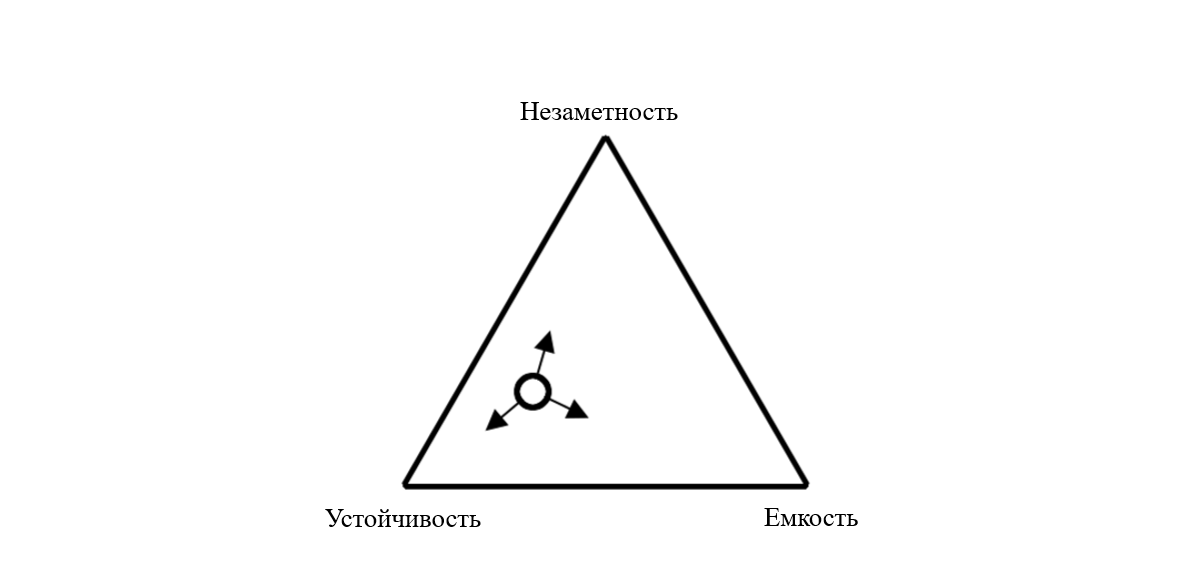
\includegraphics[width=1.0\linewidth]{Tradeoff.png}
	
	\caption{Компромисс между свойствами цифровой метки}
	
	\label{fig:tradeoff}
	
\end{figure}
\subsection{Сценарии использования и атаки на ЦВЗ}
Задачи по внедрению и извлечению ЦВЗ, как правило, рассматриваются в контексте трех сценариев: сканирование напечатанных изображений (\textit{print-scan)}, фотографирование напечатанных изображений (\textit{print-cam}), фотографирование изображений, выведенных на экран (\textit{screen-cam}).
В зависимости от сценария использования от ЦВЗ требуется устойчивость к соответствующим типам преобразований изображения. Будем называть \textit{атакой} на цифровую метку любое преобразование изображения со встроенным ЦВЗ.
Цифровая метка считается устойчивой к атаке, если после применения этой атаки сохраняется возможность определения наличия ЦВЗ и его корректного извлечения.

Атаки делятся на два класса: преднамеренные и непреднамеренные.
Под \textit{преднамеренными} атаками подразумеваются преобразования изображения человеком, знающим о наличии встроенного ЦВЗ, с целью удалить цифровую метку или изменить закодированные в ЦВЗ данные.
В данной работе такие атаки рассматриваться не будут.
\textit{Непреднамеренные} атаки включают в себя искажения изображения, возникающие в ходе соответствующего сценария.
Так, в сценарии print-scan выделяют атаки вращения, масштабирования, сдвига (rotation, scale, translation, далее RST), обусловленные различным положением бумаги в процессах печати и сканирования.
Опишем непреднамеренные атаки, характерные сценарию screen-cam.
\begin{itemize}
\item
RST.
В отличие от сценария print-scan, в сценарии screen-cam возникает пространственное вращение, поскольку камера может находится под углом к плоскости  экрана.
\item
Фокусировка.
Если камера расположена под большим углом к плоскости экрана, разные части экрана находятся на разном расстоянии от нее, поэтому часть изображения может быть не в фокусе.
\item
Неравномерная яркость фотографии.
На яркость фотографии экрана влияют несколько факторов.
Помимо того, что сам экран является источником света, на него может падать свет от других источников, или  на нем могут оказаться тени от других объектов.
На фотографии удаленные части экрана будут менее яркими, чем ближние.
\item
Эффект муара (рисунок~\ref{fig:moire}).
Этот эффект возникает из-за того, что пиксели экрана и сенсоры камеры расположены периодично.
В результате на фотографии появляется нерегулярный узор, распространяющийся по всему изображению.
\item
Сжатие фотографии.
Обычно, либо сразу после съемки, либо в процессе пересылки в сети фотографии подвергаются алгоритму сжатия (например, JPEG).
Это позволяет снимкам занимать меньше места в памяти устройства, но негативно влияет на качество изображения.
\end{itemize}
\begin{figure}[h]
	
	\centering
	
	
\includegraphics[width=1.0\linewidth]{moire.jpg}
	
	\caption{Характерный узор, возникающий из-за эффекта муара при фотографировании экрана}
	
	\label{fig:moire}
	
\end{figure}

\newpage
\section{Постановка задачи}
Необходимо разработать и реализовать метод маркирования текстовых документов, отображаемых на экране монитора, а также метод извлечения ранее встроенной информации с фотографии экрана.
ЦВЗ должен соответствовать ряду требований:
\begin{itemize}
\item
Цифровая метка должна быть незаметна для пользователя устройства
\item
Цифровая метка должна встраиваться в режиме реального времени
\item
Цифровая метка должна содержаться в любом текстовом документе, отображенном  на экране, вне зависимости от формата (например, документы Microsoft Word, документы в формате PDF, изображения сканированных документов)
\item
ЦВЗ должен быть устойчивым к атакам, возникающим в сценарии screen-cam, а именно к RST, фокусировке, неравномерной яркости, эффекту муара, сжатию фотографии
\item
Цифровая метка должна извлекаться в случае, когда на фотографии запечатлена только часть экрана
\item
Метод должен работать в режиме слепого извлечения
\end{itemize}

\newpage
\section{Обзор методов маркирования текстовых документов}
Рассмотрим предложенные ранее подходы к маркированию текстовых документов.
Алгоритмы маркирования можно разделить на три группы:
\begin{itemize}
\item
методы, основанные на формате документа,
\item
лингвистические методы,
\item
методы, работающие с документом как с изображением.
\end{itemize}

Подходы к маркированию, основанные на формате документа, встраивают ЦВЗ путем изменения характеристик формата текста, таких как размер и стиль шрифта, величина межстрочных интервалов.
Так, в работе [] биты цифровой метки встраиваются путем уменьшения или увеличения пробелов между соседними словами.
Пробелы в одной строке делятся на две равные группы (если их нечетное количество, средний пробел не рассматривается).
Далее, пробелы в одной группе увеличиваются, а в другой уменьшаются так, чтобы суммарной размер пробелов в одной строке сохранятся.
Выбор группы зависит от кодируемого бита.
Метод показал хорошие результаты по устойчивости в сценарии print-scan, однако емкость встраивания ограничена числом строк.
Подход, описанный в [], использует типы шрифта латинских букв.
Информация встраивается путем изменения шрифта заглавных букв документа на похожий.
Шрифты, доступные в программе Microsoft Word делятся на группы по 4.
Шрифт каждой из заглавных букв меняется на один из 3 похожих.
Таким образом в группе из трех заглавных букв шифруется либо буква латинского алфавита, либо пробел.

Лингвистические методы основаны на обработке естественного языка.
Для встраивания дополнительной информации используются семантические и синтаксические свойства слов.
При этом общее значение и корректность предложений не меняется.
В работе [] рассмотрено несколько грамматических конструкций английского языка, которые могут быть подвергнуты изменению без искажения содержания текста.
Например, биты цифровой метки можно кодировать изменением порядка частей предложения, соединенных союзом «и».
В статье [] описывается лингвистический подход, основанный на замене синонимичных слов.
Предложены два усовершенствования такого подхода.
Во-первых, для проверки применимости замены в данном контексте используется Google n-gram corpus [].
Во-вторых, решена проблема, возникающая из-за слов с множественным значением.
Слова языка рассматриваются как вершины графа, в котором ребрами соединены синонимы.
Каждой вершине ставится в соответствие последовательность битов, определяемая кодирующим алгоритмом.
Метод позволяет увеличить емкость встраивания для слов с большим количеством синонимов.

Методы последней группы рассматривают текстовые документы в качестве изображений.
Статистические свойства изображений, содержащих текст, существенно отличаются от свойств обычных изображений, поэтому к ним нельзя напрямую применять методы маркировки изображений, богатых цветовым разнообразием.
Основанные на изображении методы маркирования можно разделить на 2 группы: работающие в пространственном домене и работающие в доменах преобразований.

Алгоритмы встраивания, работающие в пространственном домене, внедряют ЦВЗ, изменяя распределение цветов пикселей изображения.
Например, в работе [] встраивание цифровой метки производится за счет добавления или убирания двух групп пикселей к буквам.
Группы располагаются симметрично относительно середины букв, а расстояние между группами задает кодируемый бит.
Метод обладает высокой емкостью встраивания, однако встраиваемые группы пикселей хорошо заметны.
В статье [] ЦВЗ встраивается добавлением предопределенного шаблона, состоящего из маленьких черных точек.
Шаблон множественно повторяется по всему изображению документа, благодаря чему метод устойчив к искажениям разного типа.

Подходы, работающие в доменах преобразований, перед тем как произвести маркирование применяют к изображению обратимое преобразование.
В качестве таких преобразований могут использоваться дискретное преобразование Фурье, дискретное косинусное преобразование и т.д.
Кодируемые биты встраиваются изменением частотных коэффициентов соответствующего преобразования.
В статье [] описывается метод встраивания ЦВЗ в бинарные изображения основанный на теории фракталов.
Изображение преобразуется предложенным алгоритмом фрактального кодирования.
Цифровая метка внедряется в фрактальный код специальных сегментов, обладающих определенными свойствами.
Затем проводится декодирование, результатом которого является маркированное изображение.
Большинство методов, встраивающих ЦВЗ в домены преобразований, обладают общим недостатком: они создают характерный шум на изображении, едва заметный на богатых цветами изображениях, но хорошо различимый на текстовых документах.
Такой шум может сильно исказить буквы текста, что ухудшает его читаемость (рисунок~\ref{fig:transform}).
\newpage
\begin{figure}[h]
\begin{minipage}[h]{0.48\linewidth}
\center{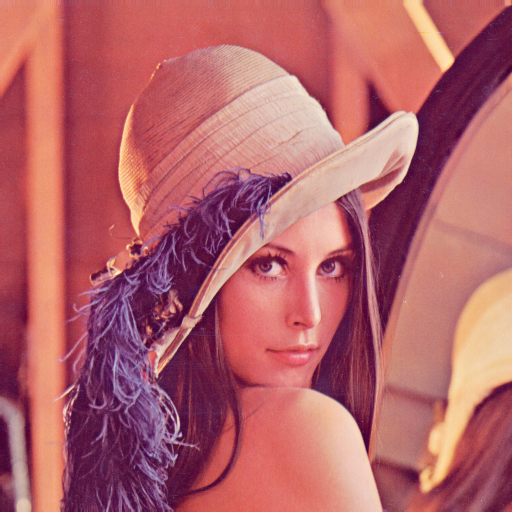
\includegraphics[width=1\linewidth]{Lenna.png}} а) Богатое цветами изображение с непериодичной структурой \\
\end{minipage}
\hfill
\begin{minipage}[h]{0.48\linewidth}
\center{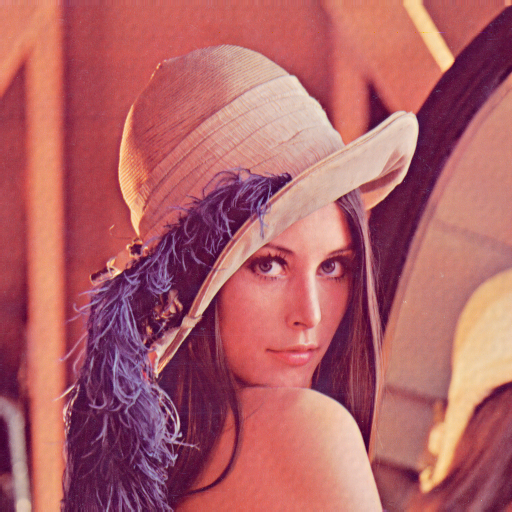
\includegraphics[width=1\linewidth]{lenna_transformed.png}} \\б) Изображение после внесения изменений в домене Фурье
\end{minipage}
\vfill
\begin{minipage}[h]{0.48\linewidth}
\center{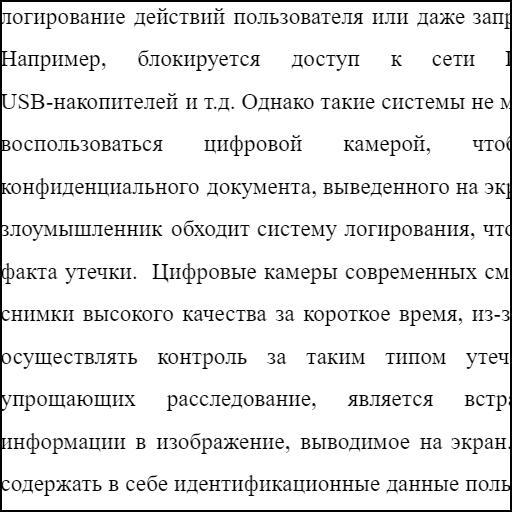
\includegraphics[width=1\linewidth]{test_doc.png}} в) Изображение текста\vspace{\baselineskip} \\
\end{minipage}
\hfill
\begin{minipage}[h]{0.48\linewidth}
\center{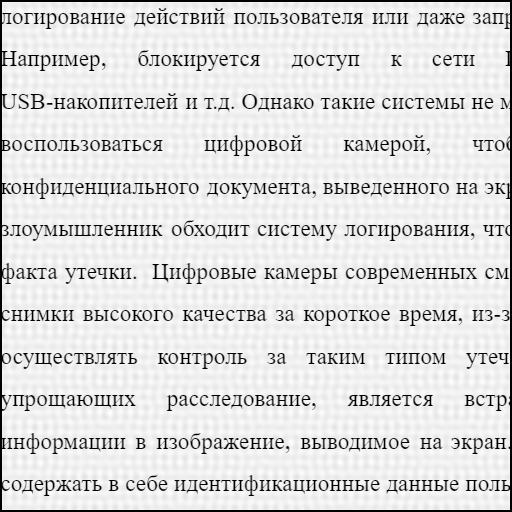
\includegraphics[width=1\linewidth]{test_doc_transformed.png}} г) Изображение текста после внесения изменений в домене Фурье \\
\end{minipage}
\caption{Сравнение изображений после внесения изменений в домене Фурье}
\label{fig:transform}
\end{figure}

\subsection{Методы, устойчивые к атакам сценария screen-cam}
За последние годы было предложено большое количество подходов к маркированию изображений.
Многие из них показали хорошие результаты устойчивости в сценарии print-scan.
Некоторые методы также неплохо проявляют себя в сценарии print-cam.
Однако большинство существующих схем внедрения ЦВЗ в изображения требуют существенных усовершенствований для успешной работы в сценарии screen-cam. 
Рассмотрим 2 метода, устойчивых к атакам в этом сценарии.

Первый подход описан в [].
Встраивание цифровой метки осуществляется в 2 этапа.
На первом этапе определяются области встраивания ЦВЗ.
Для этого используется ключевые точки, полученные с помощью алгоритма I-SIFT.
Около каждой ключевой точки выделяется прямоугольная область, в которую внедряется цифровая метка.
Кодируемая информация встраивается в домен дискретного косинусного преобразования каждой области.
Множественное повторное встраивание применяется для того, чтобы после съемки на камеру была возможность извлечь ЦВЗ из области, наименее пострадавшей от неравномерной яркости и эффекта муара.
В процессе извлечения с фотографии снова определяются ключевые точки алгоритма I-SIFT, расположение которых устойчиво к съемке.
Цифровая метка извлекается из областей около ключевых точек, определенных на фотографии.
Подход хорошо работает для большинства изображений, но не для изображений текстовых документов.
 Такие изображения обладают простой текстурой, из-за чего ключевые точки, определенные на фотографии, могут не совпадать с ключевыми точками изображения на экране. Более того, ЦВЗ внедряется в домен преобразования, что сильно сказывается на качестве отображаемого на экране текста. 

Другой метод, предложенный в [], предназначен для маркирования любого содержимого, выведенного на экран, в том числе и текстовых документов.
Подход основан на том, что зрительная система человека слабо восприимчива к небольшому непрерывному изменению яркости, в то время как камера способна его запечатлеть.
Цифровая метка встраивается путем уменьшения или увеличения яркости областей на экране.
Маска яркости, накладываемая на изображение на экране считается заранее и зависит от кодируемой информации, но не от содержимого изображения на экране.
Такой подход позволяет использовать маску в режиме реального времени, поскольку ресурсы тратятся только на ее отображение.
Авторам удалось добится работы метода в режиме слепого извлечения.
Для этого бит информации встраивается в маску в виде круга.
Область в центре делается ярче или темнее чем область у границы круга, в зависимости от значения бита.
Незаметность достигается за счет плавного изменения яркости в круге.
В процессе извлечения с фотографии определяется положение кругов и для каждого круга считается разность яркости в центре и ближе к границе.

\newpage
\section{Разработанный подход к маркированию документов}
\subsection{Встраивание ЦВЗ}
Как и в [], в предлагаемой схеме ЦВЗ встраивается в пространственный домен изображения на экране посредством изменения яркости областей на экране.
Для наложения на изображение на экране маски с областями измененной яркости используется подход, описанный в []: создается окно, обладающее свойствами визуальной прозрачности и «прозрачности» для нажатий клавиш пользователем.
Это окно всегда находится на вершине стека отображаемых окон, что позволяет встраивать ЦВЗ в любой момент времени.
Далее будем называть это окно оверлей. 
Будем рассматривать изображения как тензоры размера $W\times H\times 3$, где $W$ — ширина, $H$ — высота изображения, состоящие из пикселей в трех цветовых каналах. Пусть $I$ — изображение без учета оверлея, $OI$ — изображение в окне оверлея, $\theta$ — непрозрачность оверлея.
Тогда изображение, выводимое на экран, задается формулой:
$$SI = (1-\theta)\cdot I+\theta \cdot OI$$
С целью минимизации искажений текста и последующего упрощения определения положения ЦВЗ на снимке (на этапе извлечения ЦВЗ), цифровая метка внедряется в межстрочные интервалы.
Положение окон на экране, а также их содержимое меняется в зависимости от действий пользователя.
Содержимое оверлея необходимо постоянно обновлять, чтобы цифровая метка соответствовала измененному изображению.
Процесс встраивания ЦВЗ можно разделить на следующие этапы:
\begin{enumerate}
\item
Создание снимка экрана
\item
Очистка снимка от предыдущей цифровой метки
\item
Определение частей окон, видимых пользователем
\item
Определение областей с текстом
\item
Определение областей межстрочных интервалов
\item
Генерация шаблона яркости, соответствующего внедряемой информации
\item
Встраивание шаблона на оверлей в области, соответствующие межстрочным интервалам нижележащего маркируемого текста
\end{enumerate}
На первом этапе создается снимок экрана SI для дальнейшего определения областей с текстом.
Такой снимок содержит изображение окна оверлея $OI$, в котором отображена предыдущая метка.
Чтобы получить изображение $I$ без предыдущей метки, производится очистка по формуле:
$$I = \frac{SI- \theta\cdot OI}{1-\theta}$$

Далее определяется, какие части каждого окна видны пользователю устройства. Это делается для того, чтобы алгоритм нахождения областей с текстом применялся к каждому окну независимо от содержимого других окон.
Также важно учесть перекрытие окон.

Затем для каждого окна находятся прямоугольные области с текстом.
Поскольку маркирование производится в режиме реального времени, требуется, чтобы области с текстом находились достаточно быстро.
Высокой скоростью работы обладает метод определения областей с текстом, основанный на алгоритме FAST [].

Как и области с текстом, области межстрочных интервалов определяются по особым точкам алгоритма FAST.
Метод схож с методом определения горизонтального профиля страницы, описанным в [].
При подсчете горизонтального профиля учитываются не черные пиксели, а особые точки.
Такой подход позволяет определять области межстрочных интервалов вне зависимости от цвета текста и цвета фона.

В межстрочные интервалы встраивается шаблон яркости, пример которого изображен на рисунке~\ref{fig:template}.
Шаблон состоит из идущих подряд прямоугольных маркеров.
В начало и середину шаблона цифровой метки встраиваются специальные маркеры, состоящие из двух частей разных цветов.
Они используются в процессе извлечения ЦВЗ для определения наличия и положения цифровой метки.
Маркеры, кодирующие биты цифровой метки, встраиваются с промежутком между ними.
Темные маркеры кодируют «1», светлые — «0».
Если соседние кодирующие маркеры одинакового цвета, промежуток между ними заполняется цветом, дополняющим до белого, а если разного — средним значением цветов соседних кодирующих маркеров.
Такое чередование цветов используется для улучшения извлекаемости.
Шаблон повторяется на всю ширину текстовой области.
Ширина маркеров и количество повторений шаблона подбираются в зависимости от доли, занимаемой текстом на экране.
Затем к шаблону применяется фильтр Гаусса для сглаживания переходов яркости между маркерами.
\begin{figure}[h]
	
	\centering
	
	
\includegraphics[width=0.8\linewidth]{template.png}
	
	\caption{Шаблон яркости, встраиваемый в межстрочный интервал. Разница яркости сильно увеличена, Размытие не наложено.}
	
	\label{fig:template}
	
\end{figure}

\subsection{Извлечение ЦВЗ}
Предполагается, что описанная схема маркирования изображений будет использоваться в сценарии, в котором время, затрачиваемое на процесс извлечения, не критично.
Более того, алгоритм может быть запущен несколько раз до успешного извлечения ЦВЗ.
На вход алгоритму извлечения подается фотография текста документа или, возможно, нескольких документов, выведенных на экран.
Текст на фотографии может как содержать встроенную цифровую метку, так и не содержать.
Алгоритм извлечения ЦВЗ состоит из следующих этапов:
\begin{enumerate}
\item
Коррекция перспективы и обрезка фотографии
\item
Определение областей с текстом
\item
Определение межстрочных интервалов
\item
Удаление из межстрочных интервалов фрагментов букв
\item
Определение наличия ЦВЗ в межстрочных интервалах
\item
Извлечение ЦВЗ из межстрочных интервалов
\item
Объединение цифровых меток, извлеченных из разных межстрочных интервалов и текстовых областей.
\end{enumerate}

При фотографировании экрана камера может быть расположена под углом к плоскости экрана, поэтому на первом этапе извлечения необходимо произвести коррекцию перспективы и обрезку фотографии (рисунок~\ref{fig:perspective}).
Этот этап выполняется вручную.
\begin{figure}[h]
\begin{minipage}[h]{0.49\linewidth}
\center{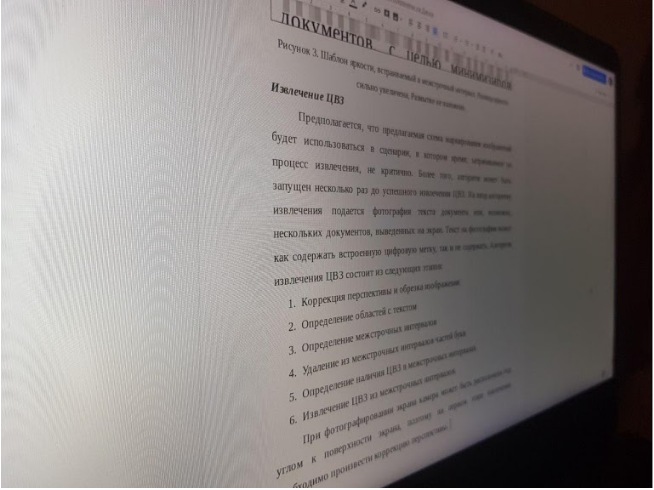
\includegraphics[width=1.0\linewidth]{perspective.png} \\ а)}
\end{minipage}
\hfill
\begin{minipage}[h]{0.49\linewidth}
\center{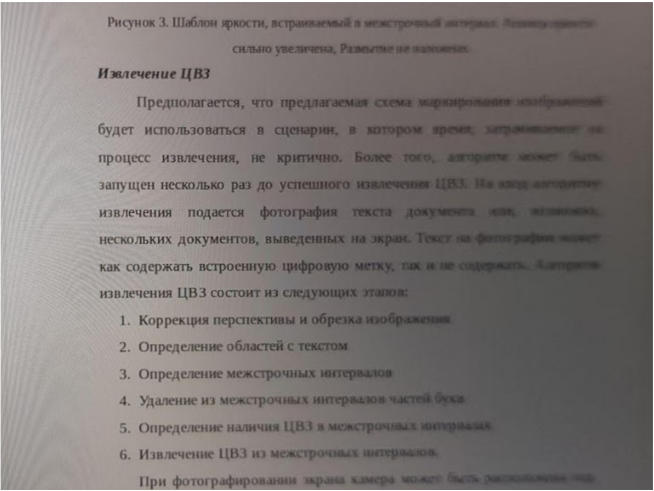
\includegraphics[width=1.0\linewidth]{perspective_corrected.png} \\ б)}
\end{minipage}
\caption{Пример коррекции перспективы и обрезки фотографии экрана}
\label{fig:perspective}
\end{figure}

На следующих двух этапах на скорректированной фотографии определяются области с текстом и межстрочные интервалы.
Для этого применяется тот же метод, что и в процессе встраивания, с той разницей, что при извлечении возможно многократное применение алгоритма с целью определить межстрочные интервалы достаточно точно.

Далее на этапе №4 из межстрочных интервалов удаляются фрагменты букв, имеющих верхние или нижние выносные элементы (например, «б», «р», заглавные буквы).
Обозначим изображение в оттенках серого рассматриваемого межстрочного интервала как функцию координат пикселей $LS(i,j); i\in[1,W],j\in[1,H]$, где $W$ — ширина, а $H$ — высота межстрочного интервала. Удаление фрагментов букв выполняется следующим образом:
$$LS(i,j) = \begin{cases}LS(i,j),\text{если } |LS(i,j) - \overline{LS}|< th\\\overline{LS}, \text{ иначе} \end{cases}$$
где $\overline{LS}$ — среднее значение яркости в межстрочном интервале,  $th$ — заданный порог.

Ранее упоминалось, что на вход алгоритму может быть передано изображение, не содержащее ЦВЗ, поэтому на следующем этапе необходимо установить факт  его наличия.
Для этого используются маркеры начала и середины метки.
Также они позволяют определить расположение метки в межстрочном интервале.
На рисунке \ref{fig:det_row} изображен график функции горизонтальной координаты $R(i)$, позволяющей получить расположение маркеров начала и середины метки. $R(i)$ задается формулой:
$$R(i) = \sum_{j=1}^HLS(i,j)\cdot\left(j - \frac{H}{2}\right), i \in [1,W]$$
\newpage
\begin{figure}[h]
\center{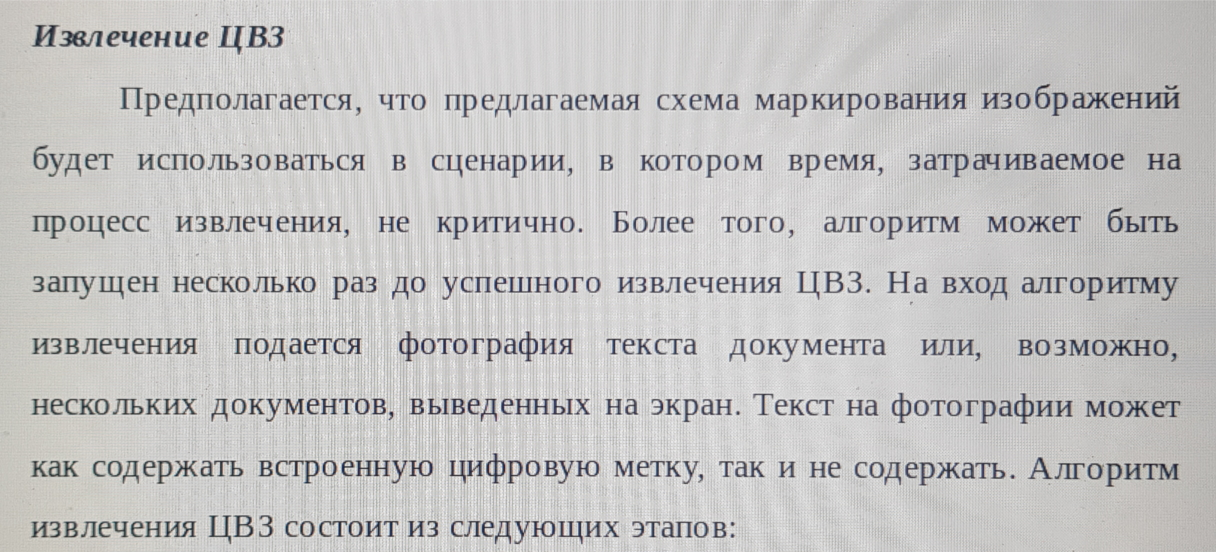
\includegraphics[width=1\linewidth]{example.jpg}} а) Фотография текста на экране со встроенным ЦВЗ \\
\center{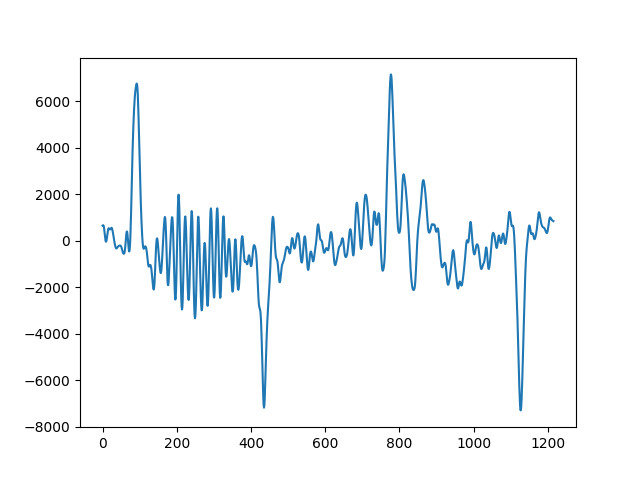
\includegraphics[width=1\linewidth]{det_row.png}} б) Сумма функций $R(i)$, полученных из межстрочных интервалов текста на фотографии а) \\
\caption{Сравнение изображений после внесения изменений в домене Фурье}
\label{fig:det_row}
\end{figure}

Поскольку кодирующие маркеры и промежутки между маркерами однотонны по вертикали, значение $R(i)$ на соответствующих позициях должно быть близко к 0.
Маркеры начала метки в нижней части ярче, чем в верхней, поэтому $R(i)$ на координатах таких маркеров достигает максимума.
Аналогично $R(i)$ достигает минимума на позициях маркеров середины метки.
Маркеры начала и середины метки, встроенные в межстрочные интервалы одной текстовой области, расположены на одинаковых позициях, поэтому экстремумы можно увеличить, просуммировав $R(i)$ разных межстрочных интервалов (рисунок~\ref{fig:det_row}).
Если в $R(i)$ можно выделить характерные максимумы и минимумы, расположенные периодично, считается, что в строке есть встроенный ЦВЗ и извлечение возможно.
Для определения периода $P$ в функции $R(i)$ применяется автокорреляционная функция (рисунок~\ref{fig:auto_correlation}):
$$AC(\tau)=\sum_{t=1}^{W} R(t)\cdot R(t-\tau)$$
\begin{figure}[h]
	
	\centering
	
	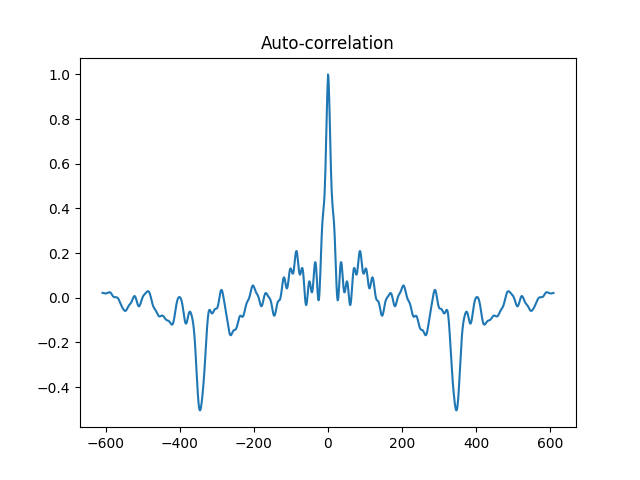
\includegraphics[width=1\linewidth]{auto_correlation.png}
	
	\caption{...}
	
	\label{fig:auto_correlation}
	
\end{figure}

Соседние экстремумы функции $R(i)$ противоположны по знаку, поэтому значение периода $P$ соответствует минимуму функции автокорреляции.
Далее для определения положения экстремумов вычисляется поэлементное произведение функции $R(i)$ на ее сдвиг на период $P$ (рисунок~\ref{fig:correlation_row}):
$$M(i)= R(i)\cdot R(i+P),\ i\in[1, W-P]$$
\begin{figure}[h]
	
	\centering
	
	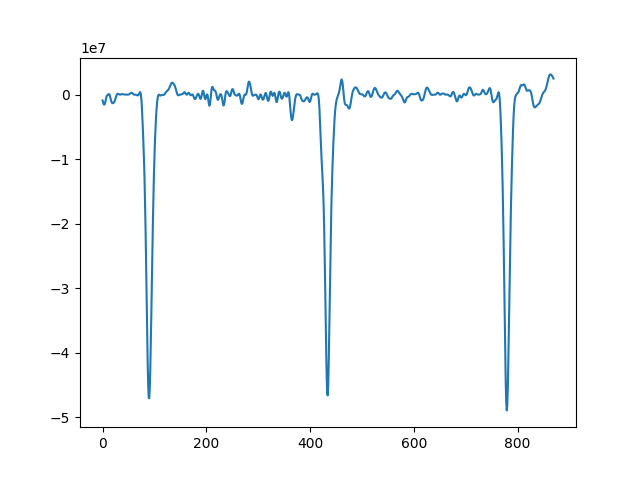
\includegraphics[width=1\linewidth]{correlation_row.png}
	
	\caption{...}
	
	\label{fig:correlation_row}
	
\end{figure}
Минимумы функции $M(i)$ расположены периодично с периодом P и соответствуют координатам экстремумов функции $R(i)$, не включая последний.
 
Зная размер встроенного сообщения и положение маркеров начала и середины метки, можно определить координаты кодирующих маркеров в межстрочном интервале.
Пусть центры кодирующих маркеров расположены на позициях $p_k$ в межстрочном интервале.
Для извлечения бита, закодированного в $k$-ом  кодирующем маркере, используется область вокруг этого маркера:
$${Area}_k(i) = \frac{1}{H}\sum_{j=1}^HLS\left(i+ \frac{p_{k-1}+p_{k}}{2},j\right),\  i\in\left[1,n_k\right],\ n_k=\frac{p_{k+1}-p_{k-1}}{2}$$
При извлечении бита метки используются следующие свойства кодирующих маркеров:
\begin{itemize}
\item
На изображении, выводимом на экран, маркеры, кодирующие бит «1», темнее, чем среднее значение яркости в межстрочном интервале, а маркеры, кодирующие «0», — светлее.
В процессе съемки возможны искажения яркости (например, при коррекции перспективы, как рисунке 4), однако такие искажения происходят на большем масштабе, чем размер одного маркера.
Восстановить исходный уровень яркости в межстрочном интервале можно путем вычитания полиномиальной аппроксимации.
Свойство отличия яркости кодирующего маркера от средней яркости межстрочного интервала можно назвать глобальным свойством маркера.
Оценка, основанная на этом свойстве, считается по формуле:
$$GS_k = \sum_{i=1}^{n_k} \left(Area_k(i)-\overline{LS}\right)$$
Отрицательное значение оценки соответствует извлекаемому биту «1», положительное — «0».
\item
При встраивании ЦВЗ пространство между кодирующими маркерами заполняется так, что положение каждого кодирующего маркера задает локальный экстремум яркости: минимум для темных маркеров и максимум для светлых.
Функция яркости от координаты оказывается выпуклой в области маркеров, кодирующих «0», и вогнута в области маркеров, кодирующих «1».
Свойство выпуклости функции яркости в области кодирующего маркера можно назвать локальным свойством маркера.
Оценка выпуклости вычисляется по формуле:
$$CS_k=\sum_{i=1}^{n_k}\left(Area_k(j)-\left(\frac{Area_k(n_k)-Area_k(1)}{n_k-1}\cdot (i-1) + Area_k(1)\right)\right)$$
\end{itemize}
Полученные оценки суммируются с коэффициентом $\alpha$:
$$S_k = {GS}_k +\alpha \cdot {CS}_k$$

Каждому биту цифровой метки могут соответствовать несколько кодирующих маркеров, находящихся в разных межстрочных интервалах и текстовых областях.
Оценки, полученные при извлечении маркеров, кодирующих тот же бит,  суммируются.
Знак суммы отвечает за значение извлекаемого бита, а модуль характеризует степень уверенности в этом значении.
\newpage
\section{Результаты}
Был проведен ряд экспериментов с целью определить оптимальные параметры предложенного метода.
Для оценки извлекаемости цифровой метки применяется мера Bit Error Rate (далее, BER) [].
BER считается как отношение числа неверно извлеченных бит к общему числу бит цифровой метки. Для сравнения результатов работы алгоритма извлечения предлагаемого подхода также используется качественная оценка:
$$ES = \sqrt{\frac{N}{\sum_{k = 1}^{N}\frac{1}{S_k^2}}},$$ 
где суммирование проводится по всем значениям $S_k$, соответствующим битам извлеченной цифровой метки.
Эта оценка зависит от параметров изображения, подаваемого на вход алгоритма извлечения, поэтому фотографии экрана, используемые при тестировании, приводятся к единому формату.

Все тесты проводились с использованием монитора AOC-i2769Vm [] диагональю 27 дюймов и с разрешением $1920\times 1080$ пикселей.
Снимки экрана производились на камеру смартфона Samsung Galaxy S8 [], обладающую характеристиками: 12 мегапикселей, апертура f/1.7, фокусное растояние 26 мм.
\subsection{Непрозрачность маркеров}

\end{document}